\begin{frame}{Extraction de la terminologie : approche linguistique $\cdot$ \texttt{TermSuite}\footnote{\url{https://termsuite.github.io/}}\textsuperscript{,}\footnote{\url{https://github.com/ljpetkovic/Charcot\_TermSuite/tree/main}}}
	%	Corpus Charcot accessible sur la plateforme \textsc{OBVIE} \hfill {\small\citep{alrahabi2022obvie}}
	%	\begin{itemize}
		%		\item fouille avancée des corpus en \textsc{XML-TEI}
		%		\item textes similaires : mots fréquents / en commun, noms cités
		%	\end{itemize}
	%	%\danger impossible de quantifier l'importance des MWEs
	%	\begin{figure}[!h]
		%		\centering
		%		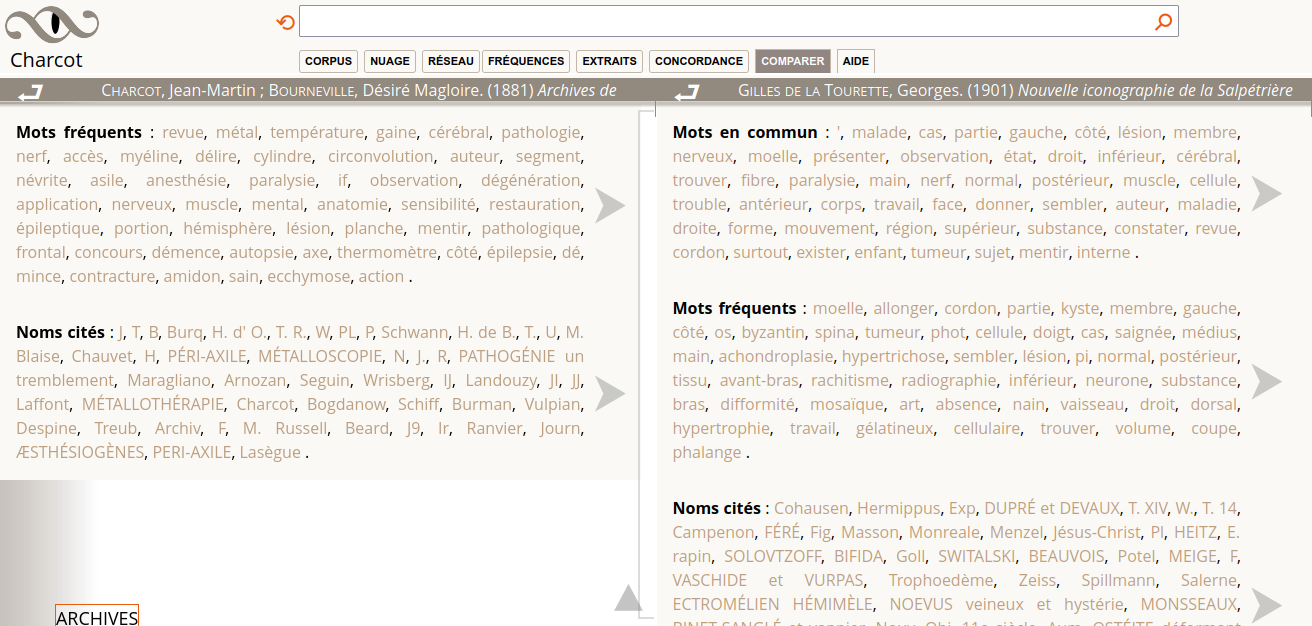
\includegraphics[width=90mm,scale=0.5]{pic/doc_sim.png}
		%		\caption{Points similaires entre un ouvrage de Charcot et celui de de la Tourette.}
		%		%    \caption{Distribution des fréquences des tokens avec la frise chronologique pour ceux constituant l'expression \textit{bulbe rachidien} (issus des corpus \og{}Charcot\fg{} et \og{}Autres\fg{}).}
		%		\label{fig:my_label}
		%	\end{figure}
	%Mesurer informatiquement l'impact de Charcot sur son \og{}réseau\fg{} \\$\rightarrow$ intertextualité uni-directionnelle
	%\begin{figure}[!h]
	%    \centering
	%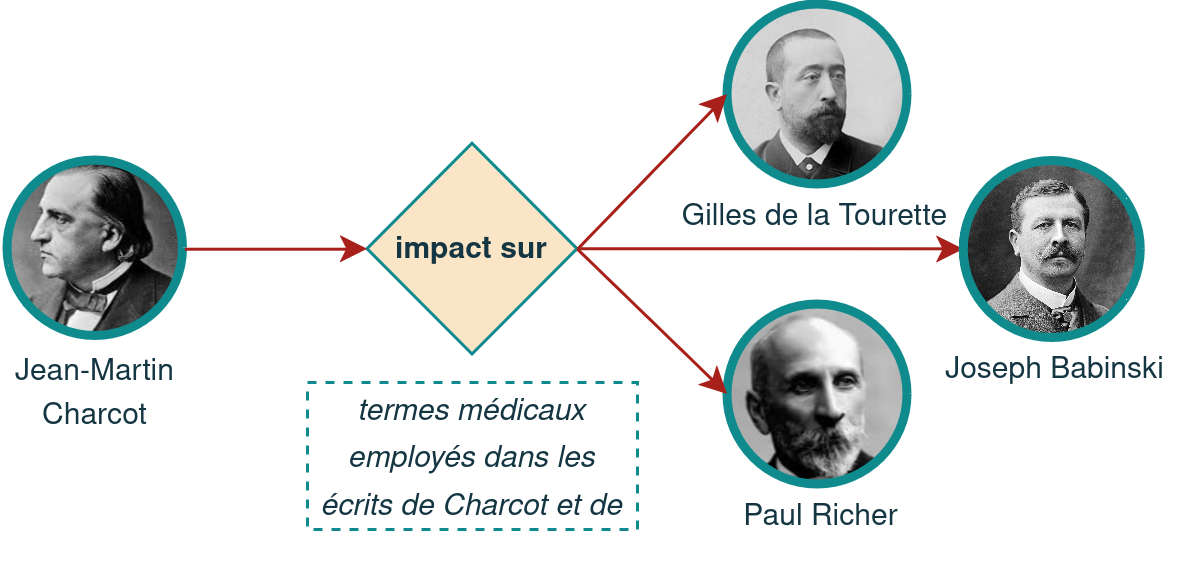
\includegraphics[width=100mm,scale=0.5]{pic/charcot_intertextualite.png}
	%    \caption{Opérationnalisation de l'impact de Charcot sur ses élèves.}
	%    \label{fig:my_label}
	%\end{figure}
	%	\begin{variableblock}{\texttt{TermSuite}\footnote{\url{https://termsuite.github.io/}}}{bg=white,fg=deepblue}{bg=white,fg=deepred}
		%		\justifying
		%%	Extraction des termes uniques et de leurs caractéristiques \begin{itemize}
			%%		\item étiquettes \textsc{POS}, fréq. brute et documentaire,  \textsc{TF-IDF}, spécificité$\dots$
			%%	\end{itemize}
		%\end{variableblock}
		Termes uniques + motifs syntaxiques (6)
		\begin{itemize}
			\item système à base de règles + mesures statistiques
			\begin{itemize}
				\item \textsc{TF-IDF}, spécificité, fréquences$\dots$
				\item 261 termes en commun
			\end{itemize} 
		\end{itemize}
		\begin{table}[h]
			\centering
			\resizebox{\textwidth}{!}{
				\begin{tabular}{|lrrr|rrl|}
					\hline\hline
					\rowcolor{gray!10}\multicolumn{4}{|c|}{Corpus Charcot}                                                                    & \multicolumn{3}{|c|}{Corpus Autres}                               \\ \hline
					\multicolumn{1}{|c|}{Motif POS}      & \multicolumn{1}{c|}{Effectif} & \multicolumn{1}{c|}{Fréq. relat. (\%)} & \multicolumn{1}{c|}{Exemple} & \multicolumn{1}{c|}{Effectif} & \multicolumn{1}{c|}{Fréq. relat. (\%)} & \multicolumn{1}{c|}{Exemple}\\ \hline
					\rowcolor{yellow!30}\multicolumn{1}{|c|}{\textsc{N}}              & \multicolumn{1}{r|}{261}               & \multicolumn{1}{r|}{52,10}                   & \multicolumn{1}{c|}{\textit{hystérie}} & \multicolumn{1}{r|}{271}               & \multicolumn{1}{r|}{54,20} & \multicolumn{1}{c|}{\textit{somnambule}}                  \\ \hline
					\multicolumn{1}{|c|}{\textsc{A}}              & \multicolumn{1}{r|}{151}               &  \multicolumn{1}{r|}{30,14}                   & \multicolumn{1}{c|}{\textit{cérébral}} & \multicolumn{1}{r|}{149}               & \multicolumn{1}{r|}{29,80}      &   \multicolumn{1}{c|}{\textit{hypnotique}}          \\ \hline
					\multicolumn{1}{|c|}{\textsc{N A}}            & \multicolumn{1}{r|}{73}                & \multicolumn{1}{r|}{14,57}                   &
					\multicolumn{1}{c|}{\textit{système nerveux}} 	& \multicolumn{1}{r|}{73}                & \multicolumn{1}{r|}{14,60}       	&
					\multicolumn{1}{c|}{\textit{lame médullaire}}            \\ \hline
					\multicolumn{1}{|c|}{\textsc{N P N}}          & \multicolumn{1}{r|}{12}                & \multicolumn{1}{r|}{2,40}                    &
					\multicolumn{1}{c|}{\textit{cas de folie}} &
					\multicolumn{1}{r|}{6}                 & \multicolumn{1}{r|}{1,20}   &
					\multicolumn{1}{c|}{\textit{scissure de sylvius}}                 \\ \hline
					\multicolumn{1}{|c|}{\textsc{N A A}}          & \multicolumn{1}{r|}{3}                 & \multicolumn{1}{r|}{0,60}                    &
					\multicolumn{1}{c|}{\textit{système nerveux central}} &
					\multicolumn{1}{r|}{0}                 & \multicolumn{1}{r|}{0,00}           &
					\multicolumn{1}{c|}{--}         \\ \hline
					\multicolumn{1}{|c|}{\textsc{R}}              & \multicolumn{1}{r|}{1}                 & \multicolumn{1}{r|}{0,20}                    &
					\multicolumn{1}{c|}{\textit{[d']emblée}} &
					\multicolumn{1}{r|}{1}                 & \multicolumn{1}{r|}{0,20}       &
					\multicolumn{1}{c|}{\textit{obliquement}}             \\ \hline\hline
					\multicolumn{1}{|c|}{\textbf{Total}} & \multicolumn{1}{r|}{\textbf{501}}      & \multicolumn{1}{r|}{100,00}                  &
					\multicolumn{1}{r|}{\cellcolor{blue!25}} &
					\multicolumn{1}{r|}{\textbf{500}}      & \multicolumn{1}{r|}{100,00} &
					\multicolumn{1}{r|}{\cellcolor{blue!25}}                 \\ \hline\hline
				\end{tabular}
			}
			\caption{Répartition des parties du discours constituant les termes médicaux dans les deux corpus.}
			\label{tab:repartition_POS}
		\end{table}
	\end{frame}
	
	
	\begin{frame}{Répartition des motifs syntaxiques}
		
		\begin{itemize}
			\item unigrammes de noms \texttt{[N]} et des adjectifs \texttt{[A]} : les plus fréquents
			\item trigrammes : les séquences les plus longues extraites
			\begin{itemize}
				\item aucune occurrence du trigramme \textit{sclérose latérale amyotrophique}\\\textcolor{deepred}{seule trace : adjectif \texttt{[A]} \textit{latérale}}
				\item \textit{idem} pour le quadrigramme \textit{état de mal hystéro-épileptique}
			\end{itemize}
			
		\end{itemize}
		
		\begin{figure}[!h]
			\centering
			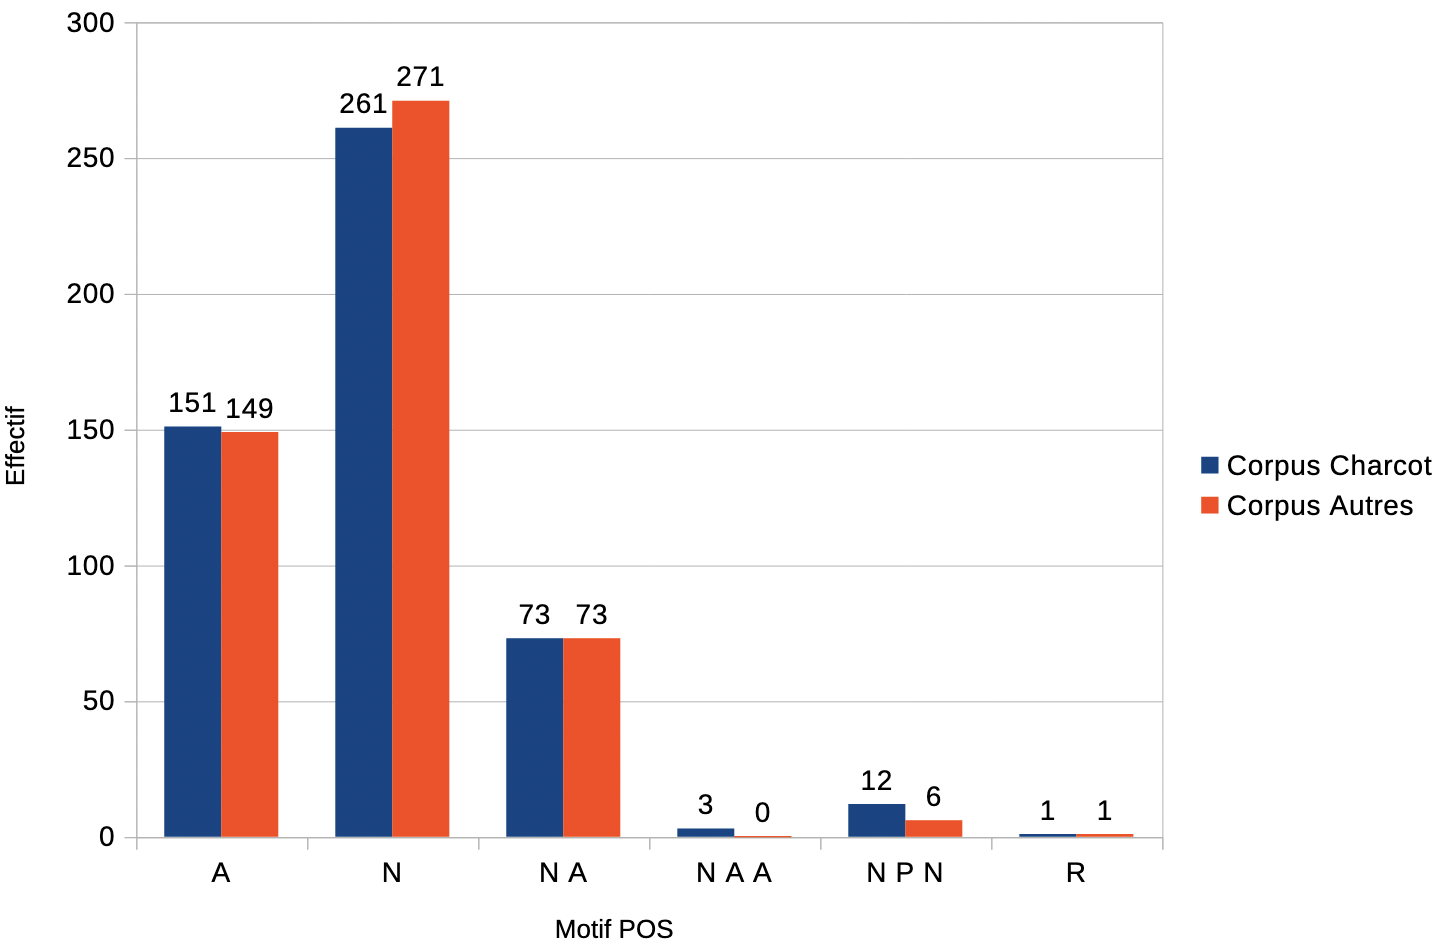
\includegraphics[width=0.65\textwidth]{pic/repartition_motifs_POS.png}
			\caption{Analyse comparative des séquences syntaxiques.}
		\end{figure}
		
	\end{frame}
	
	\begin{frame}{\textsc{TF-IDF}}
		Premiers 12 termes communs, à partir du \texttt{TF-IDF} $\approx$ \textsc{0,15}
		\begin{itemize}
			\item prévalence des unigrammes
		\end{itemize}
				\begin{figure}[!h]
			\centering
			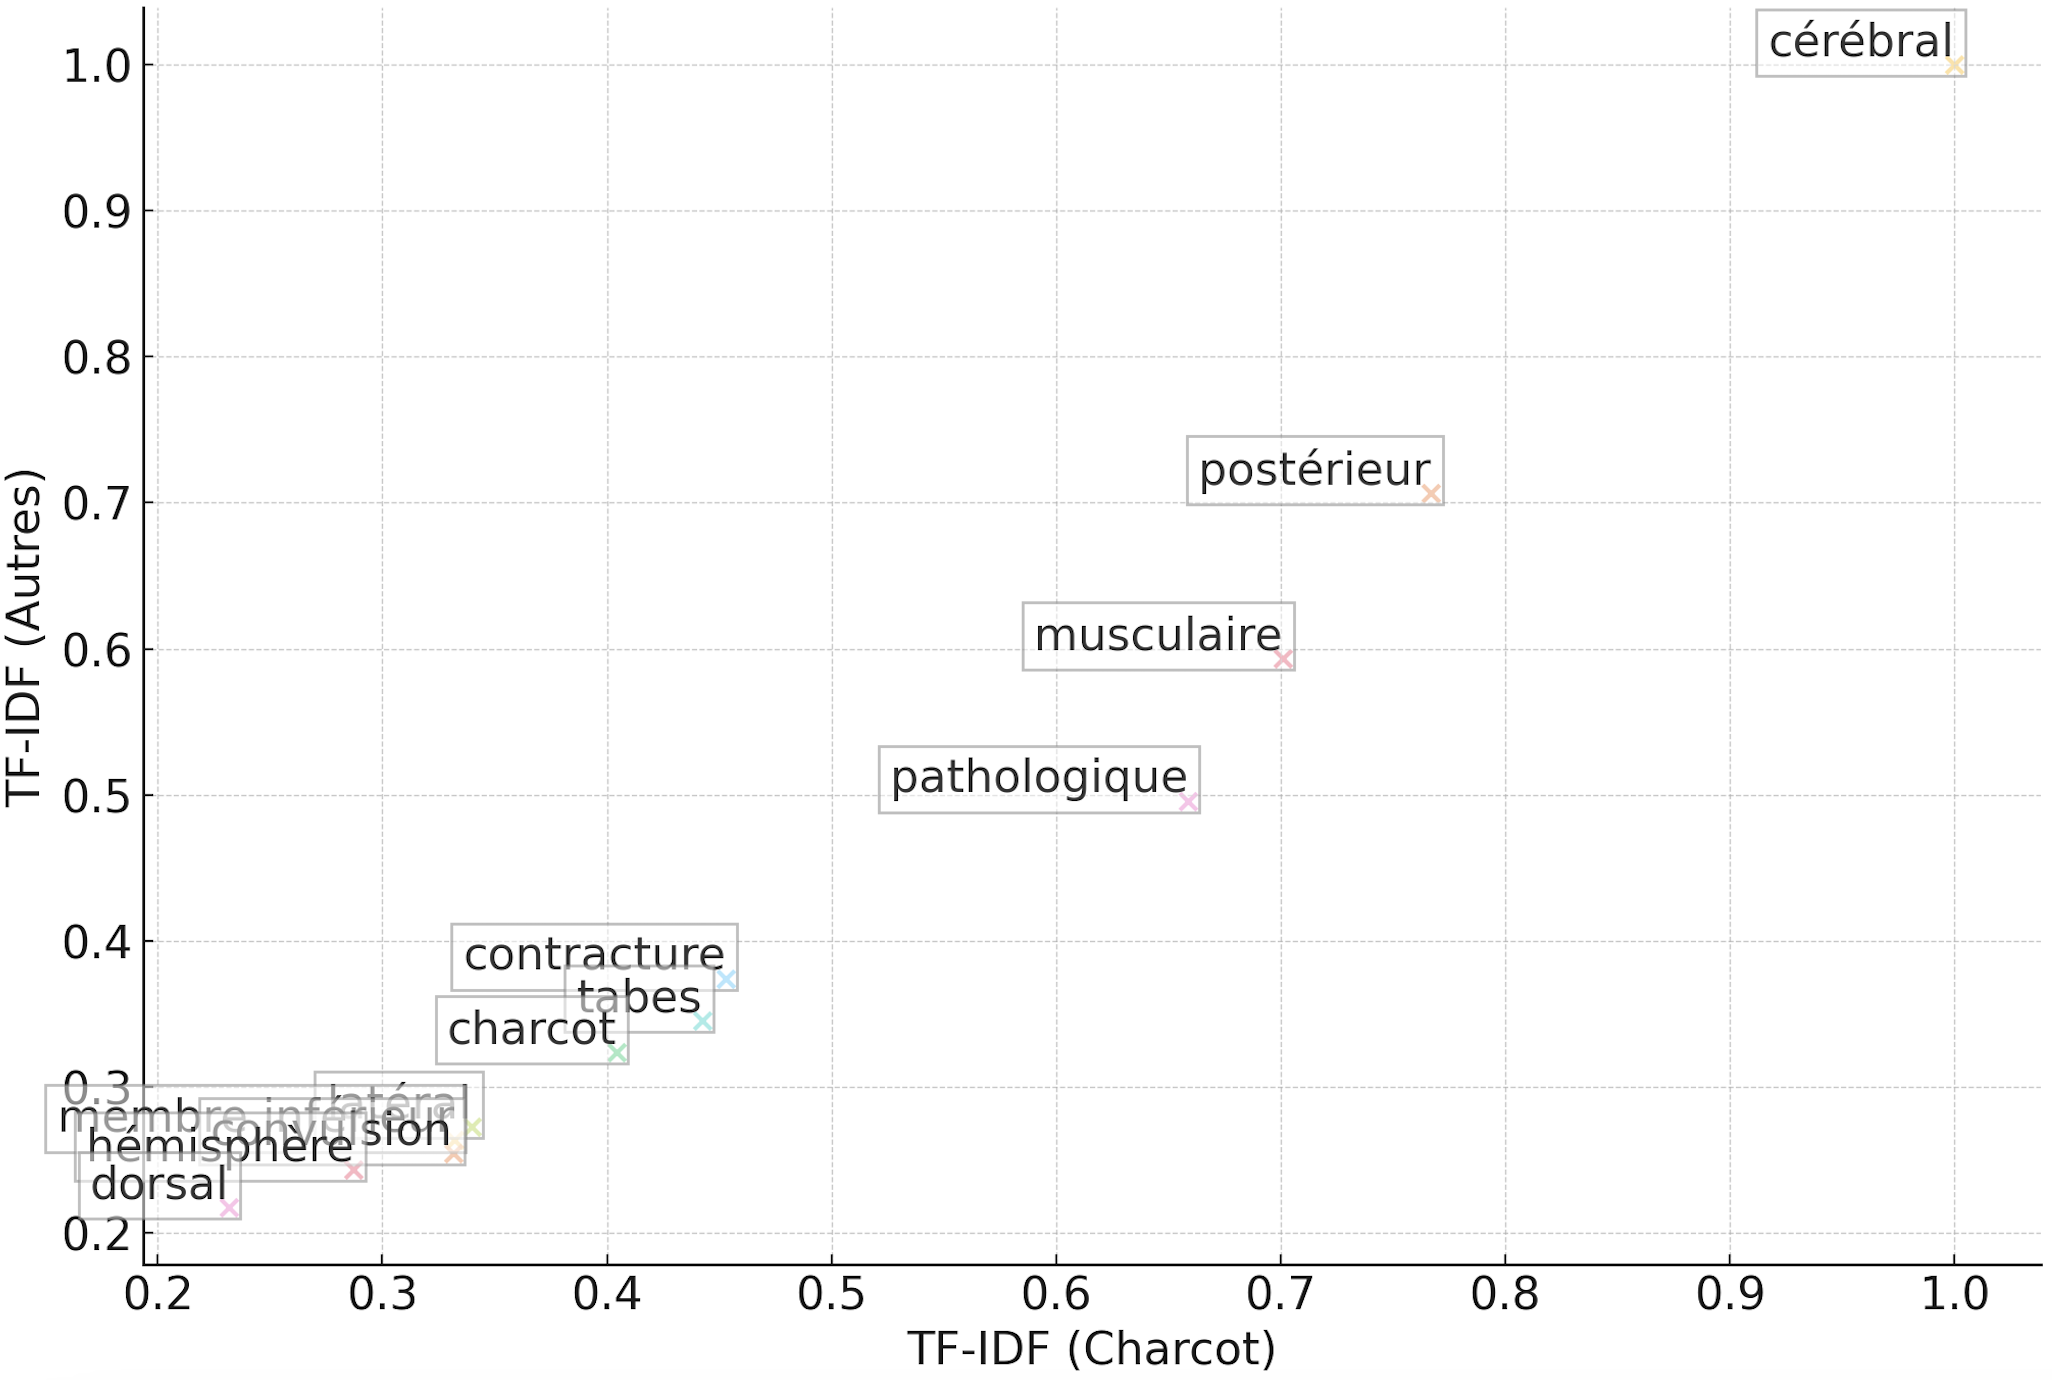
\includegraphics[width=0.7\textwidth]{pic/scatter_plot.png}
			\caption{Termes communs avec leurs valeurs \textsc{TF-IDF} respectives.}
		\end{figure}
	\end{frame}

%\begin{frame}{Corpus Charcot -- \textsc{OBVIE}}
%	
%	\begin{itemize}
%		\item Fonds Charcot sur SorbonNum\footnote{\url{https://patrimoine.sorbonne-universite.fr}}
%		\item Corpus Charcot sur \textsc{OBVIE}\footnote{\url{https://obtic.huma-num.fr/obvie/charcot/?view=corpus}}
%	\end{itemize}
%	
%	
%\end{frame}

%\begin{frame}{Extraction des phrases-clés $\cdot$ méthode supervisée}
%	\begin{figure}[!h]
%		\centering
%		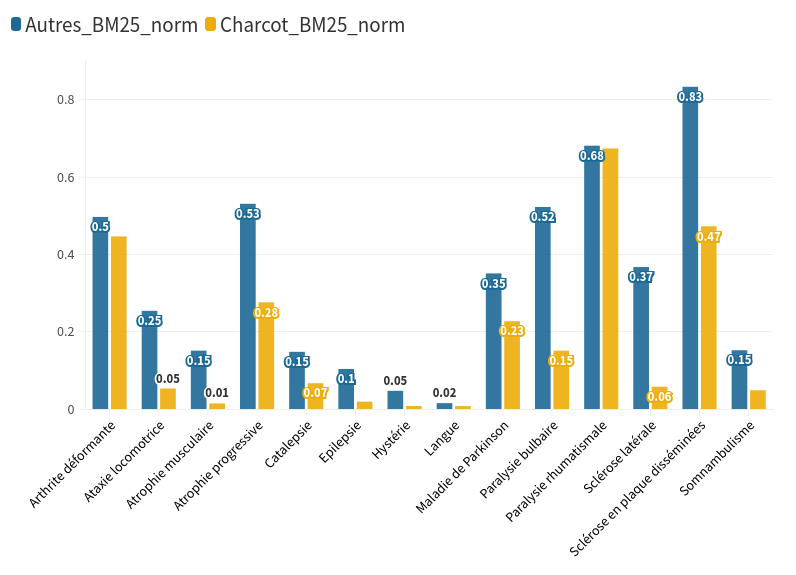
\includegraphics[width=0.6\textwidth]{pic/Charcot_Autres_250523.png}
%		\caption{Visualisation de pertinence des concepts dans les deux corpus suivant la métrique \textsc{BM25} \citep{robertson1976relevance}.}
%	\end{figure}
%	\textsc{BERT} \citep{vaswani2023} : diplopie, myélite partielle$\dots$ (Charcot)\\
%	\quad\quad\quad vicieuses, délire, miracle$\dots$ (Autres)
%\end{frame}

%\begin{frame}{Extraction des phrases-clés $\cdot$ méthode non-supervisée}
%	\begin{figure}[!h]
%		\centering
%		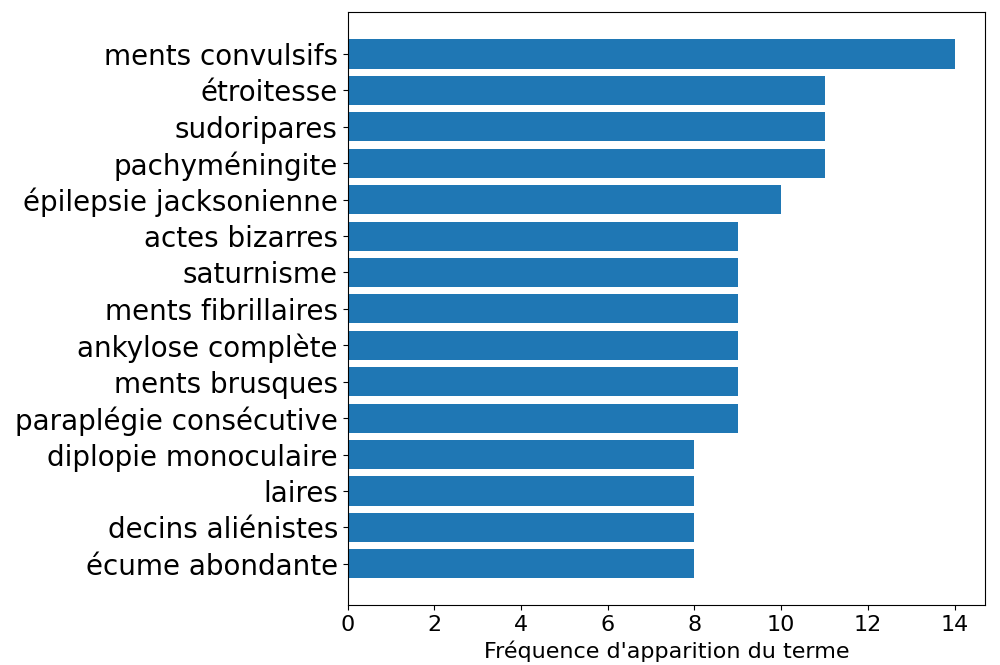
\includegraphics[width=0.8\textwidth]{pic/termes_partages.png}
%		\caption{Les 15 termes les plus fréquents partagés par Charcot et son réseau selon \texttt{keyphrase-vectorizers}\footnote{\url{https://pypi.org/project/keyphrase-vectorizers/}}.}
%	\end{figure}
%\end{frame}